\begin{frame}{Legenda}
    \begin{quote}
        \quad Pod kopułą świątyni Brahmy w Benares znajduje się tablica z brązu, na której umieszczone są trzy diamentowe słupki. Na jednym z tych słupków Bóg umieścił sześćdziesiąt cztery krążki z czystego złota. W ten sposób powstała wieża z Brahmy. \\
        \quad Dniem i nocą mnisi z pobliskiego klasztoru przekładają krążki z jednego diamentowego słupka na drugi zgodnie z wyznaczonymi regułami. \\
        \quad Kiedy wszystkie sześćdziesiąt cztery krążki zostaną przeniesione ze słupka, na którym umieścił je Bóg, na inny słupek, to wszystko - słupki , wieża, świątynia i mnisi - zamieni się w pył i cały świat ulegnie zniszczeniu.
    \end{quote}
\end{frame}
\begin{frame}{Działanie}
    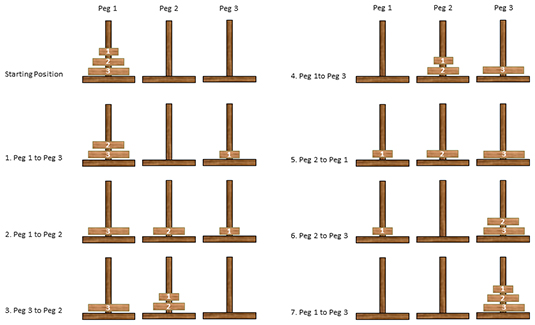
\includegraphics[width=\textwidth,height=0.8\textheight]{recursion/graphics/hanoi_tower.jpg}
\end{frame}
\begin{frame}[fragile]{Kod w Pythonie}
    \lstinputlisting{recursion/code/hanoi.py}
\end{frame}
\begin{frame}{Wynik działania kodu}
    \centering
    Moving 1th disk from A to C using B as assistant\\
    Moving 2th disk from A to B using C as assistant\\
    Moving 1th disk from C to B using A as assistant\\
    Moving 3th disk from A to C using B as assistant\\
    Moving 1th disk from B to A using C as assistant\\
    Moving 2th disk from B to C using A as assistant\\
    Moving 1th disk from A to C using B as assistant\\
    Moving 4th disk from A to B using C as assistant\\
    Moving 1th disk from C to B using A as assistant\\
    Moving 2th disk from C to A using B as assistant\\
    Moving 1th disk from B to A using C as assistant\\
    Moving 3th disk from C to B using A as assistant\\
    Moving 1th disk from A to C using B as assistant\\
    Moving 2th disk from A to B using C as assistant\\
    Moving 1th disk from C to B using A as assistant\\
\end{frame}
\begin{frame}{Wielkość problemu}
    Dla każdej kolejnej wartości problem jest dwa razy większy - liczy się dwa razy dłużej. \\
    h(n) to ilość koniecznych do wykonania przemieszczeń pojedyńczego dysku dla n-dużego problemu. \\
    \[ h(1) = 1 \]
    \[ h(n) = h(n-1) + 1 + h(n-1) \]
    \[ h(n) = 2 \cdot h(n-1) + 1 \]
    \[ H(n) = h(n) + 1 = 2(h(n-1) + 1) \]
    \[ H(n) = 2 \cdot H(n-1) \]
    \[ H(1) = 2 \]
    \[ H(n) = 2^n \]
    \[ h(n) = 2^n - 1 \]
\end{frame}
\begin{frame}{Wielkość problemu}
    Problem rośnie wykładniczo, podobnie jak w legendzie o wynalezieniu szachów. Wzór na liczbę ziarenek (ciąg geometryczny o $a_1=1, q=2$) na n-tym polu wynosi $r(n) = 2^{n-1}$. \\
    Wzór na sumę wszystkich ziarenek (suma pierwszych wyrazów ciągu) do n-tego pola włącznie wynosi:
    \[ S_r(n) = a_1 \cdot \frac{1-q^n}{1-q} = 1 \cdot \frac{1-2^n}{1-2} = 2^n - 1 \]
    \centering
    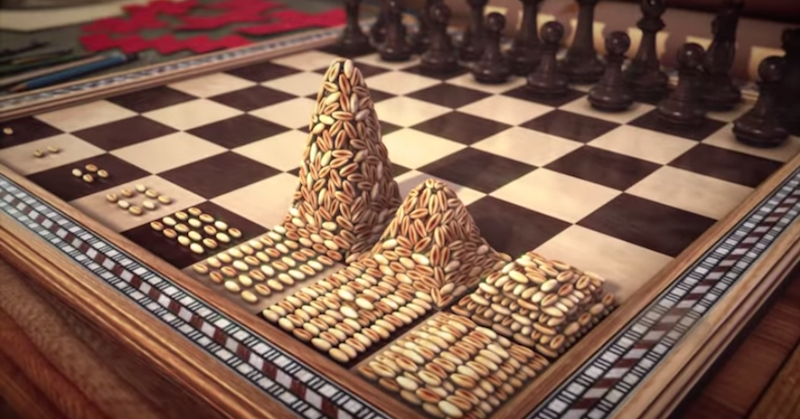
\includegraphics[height=0.35\textheight]{recursion/graphics/chessboard1.png}
\end{frame}
\begin{frame}{Wielkość problemu}
    \centering
    \begin{columns}
        \begin{column}{0.5\textwidth}
            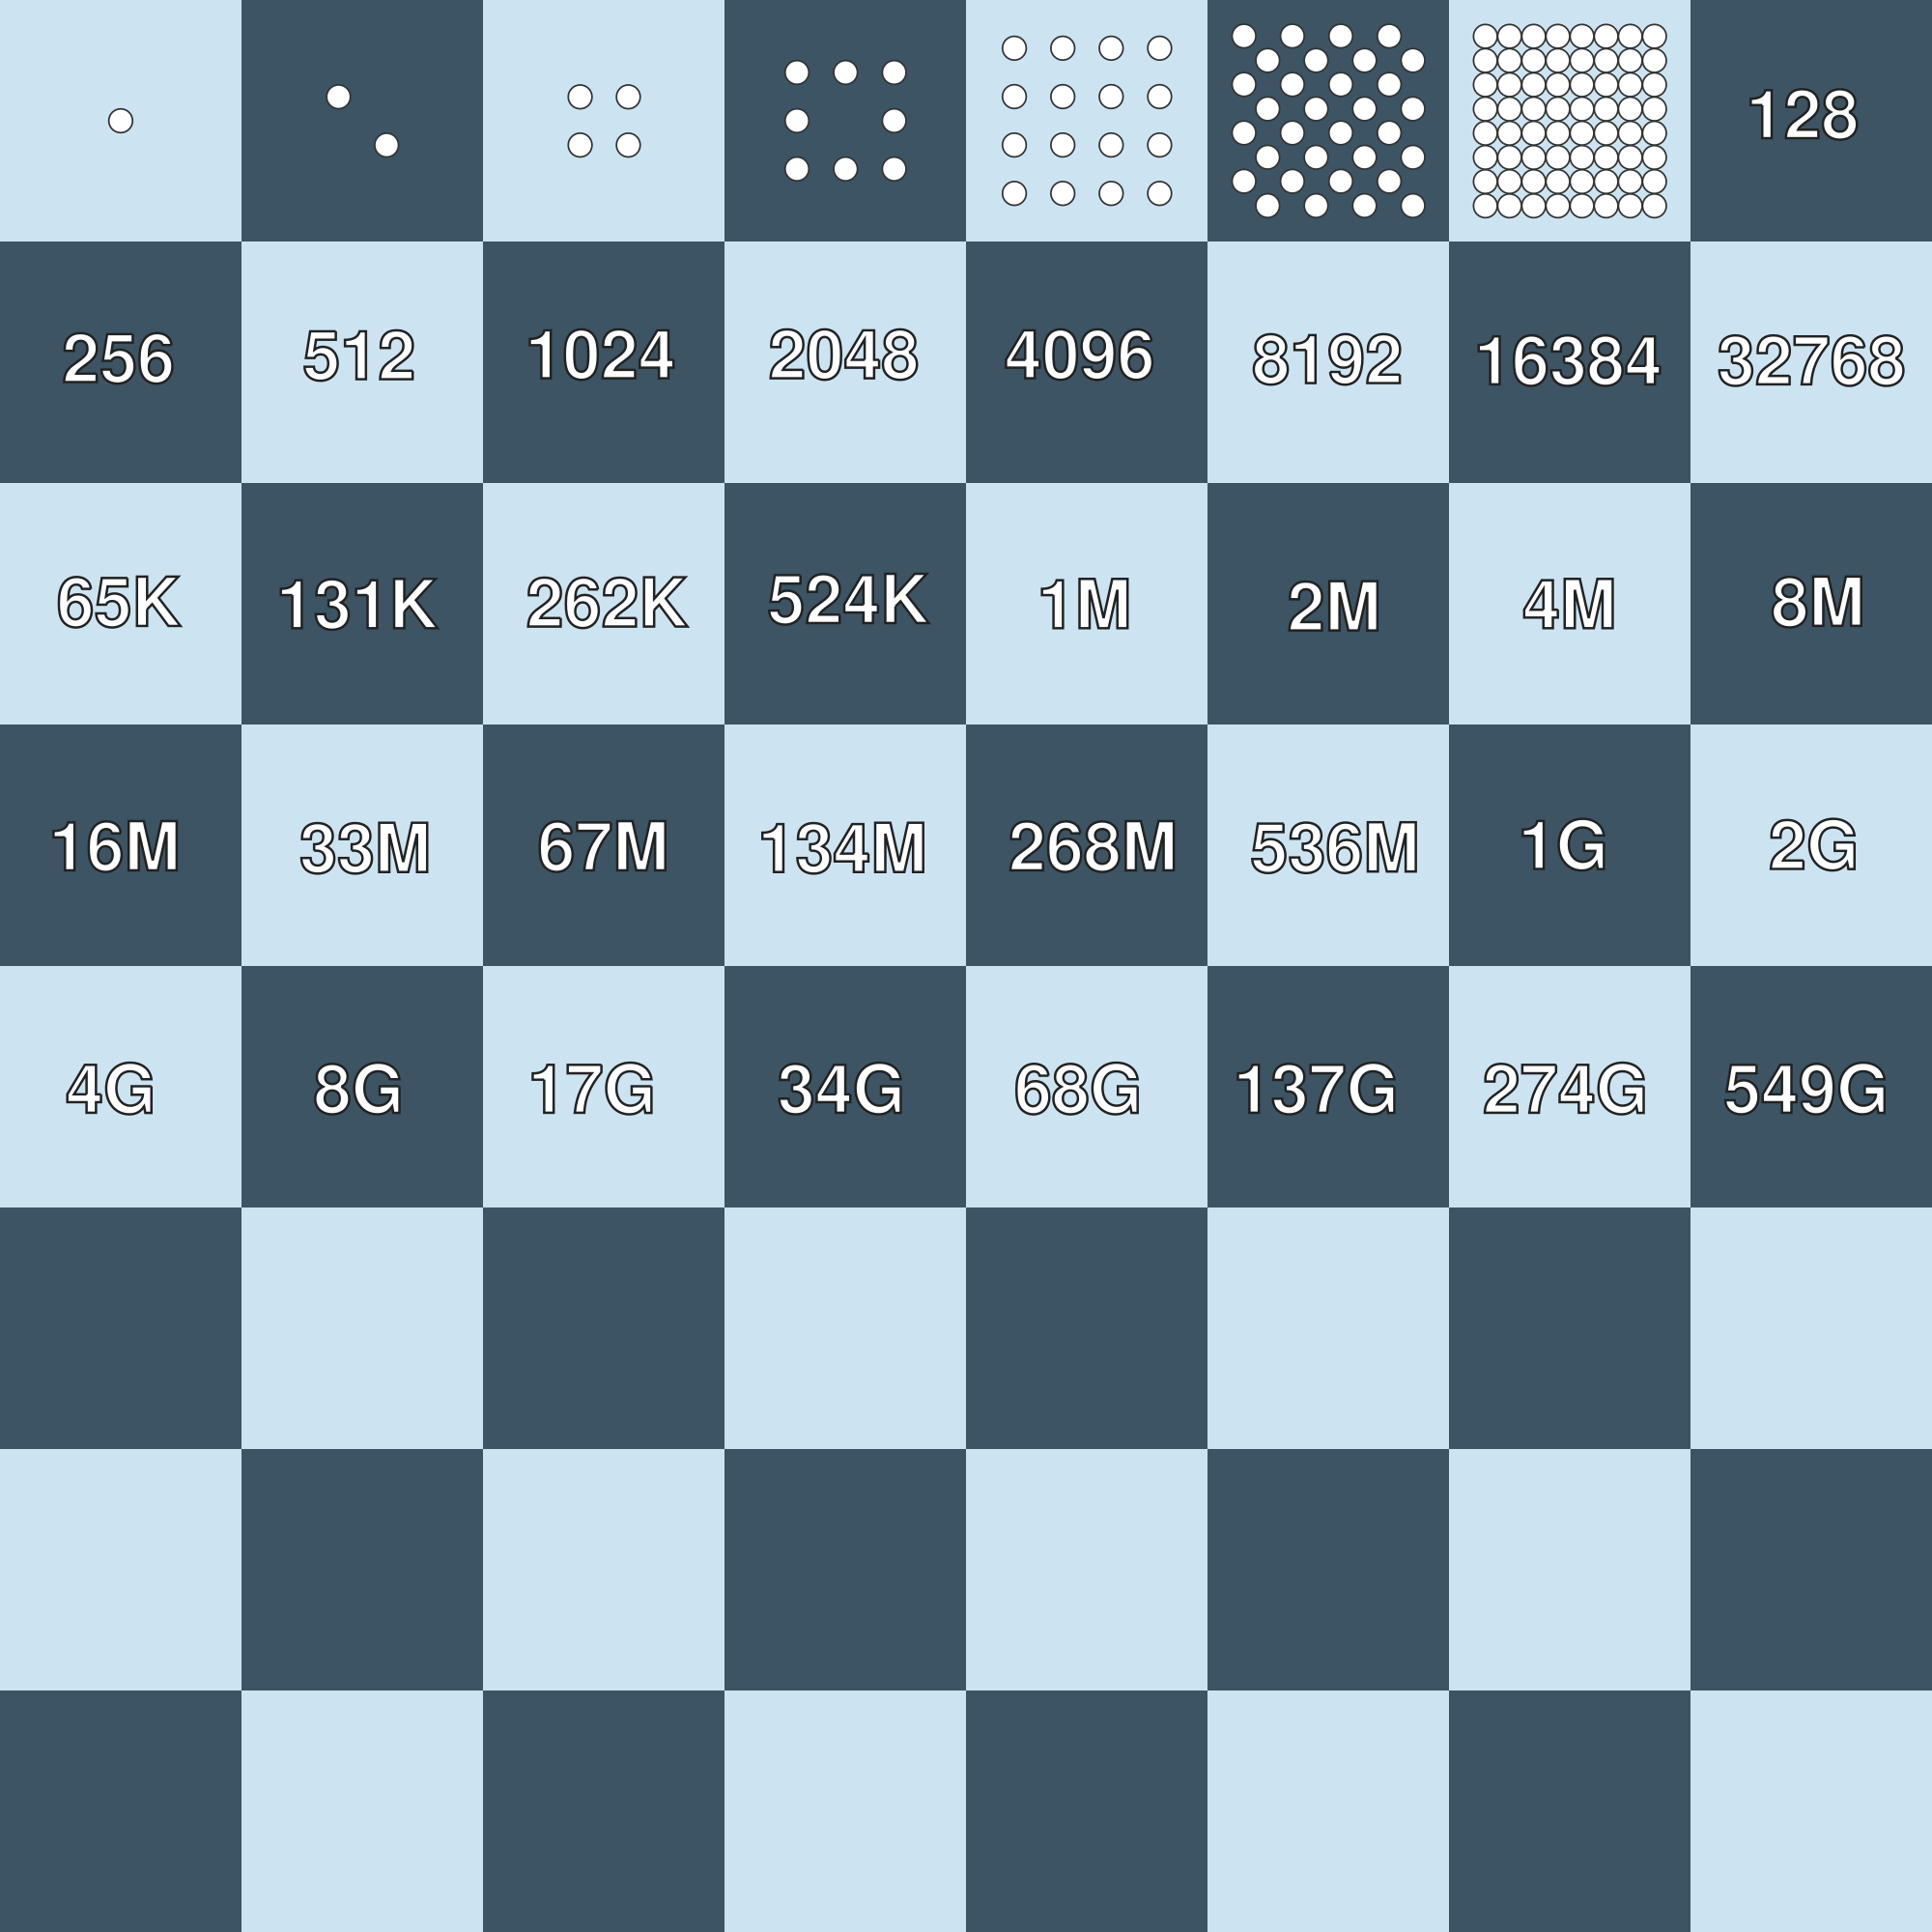
\includegraphics[height=0.7\textheight]{recursion/graphics/chessboard2.png}
        \end{column}
        \begin{column}{0.5\textwidth}
            W przypadku szachownicy mamy łącznie na wszystkich 64 polach $S_r(64)$ ziarenek ryżu. \\
            W przypadku wieży hanoi dla 64 dysków mamy $h(64)$ koniecznych przesunięć.
            \[ S_r(64) = 2^{64} - 1 = h(64) \]
            \[ 2^{64} - 1 = 18.446744 \cdot 10^{18} \]
        \end{column}
    \end{columns}
\end{frame}